\documentclass{beamer}

\usepackage[game]{sfocs-slides}

\author{Team $13$:Qiao Liu, Yifan Jia, Zining Wang}
\title{}
\date{Summer 2021}

\begin{document}

\maketitle

\section{Multiple images on a slide}

\begin{frame}{Two pictures}
	
	\begin{tikzpicture}[overlay, remember picture]

		\node[anchor=south east,outer sep=0pt,inner sep=0pt] (c1) at (current page.south east)  {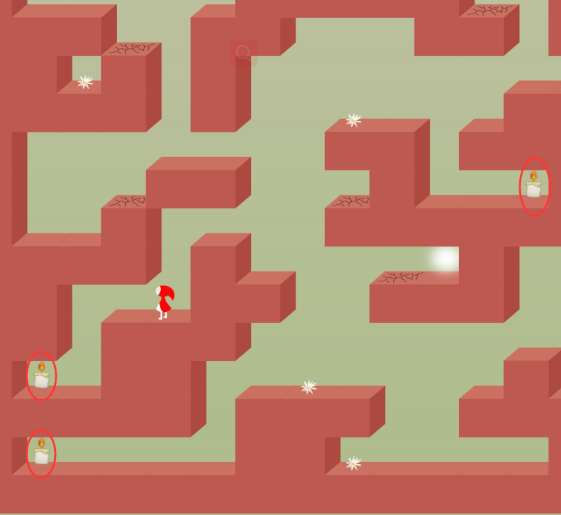
\includegraphics[height=\heightii]{candle1}};
		\node[anchor=south east,outer sep=0pt,inner sep=0pt] at (c1.north east) (c2) {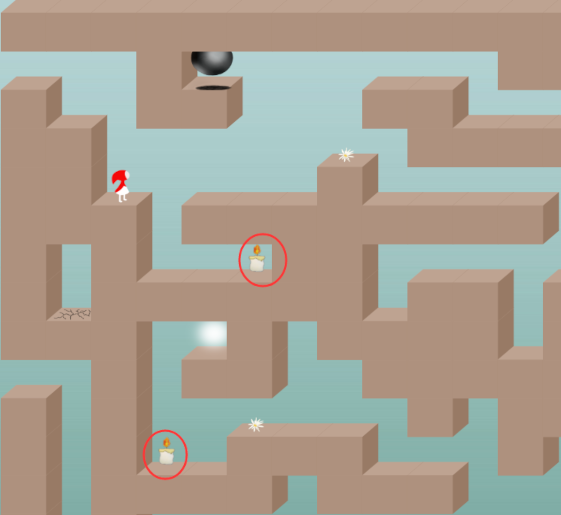
\includegraphics[height=\heightii]{candle2}};

	\end{tikzpicture}

	\begin{columns}
		\column{.5975\textwidth}
		Comments:
		\begin{itemize}\bigsep
			\item Two pictures
			\item On the right (east)
			\item Bullet points should occupy the space
			\item Column width should be adjusted
		\end{itemize}

		\column{.35\textwidth}

	\end{columns}

\end{frame}

\begin{frame}{Three pictures}

	\begin{tikzpicture}[overlay, remember picture]

		\node[anchor=south west,outer sep=0pt,inner sep=0pt] (c1) at (current page.south west)  {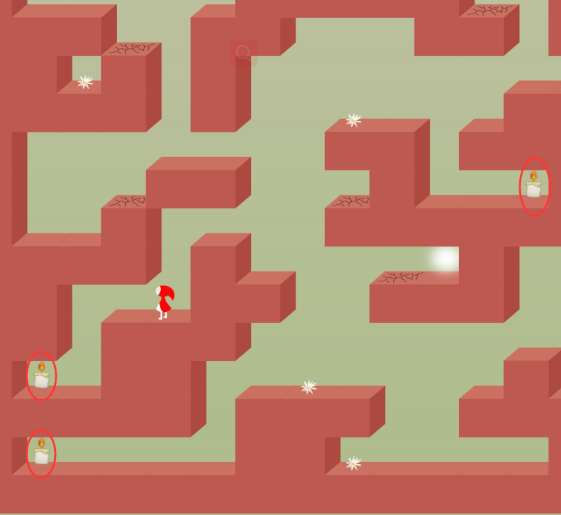
\includegraphics[height=\heightiii]{candle1}};
		\node[anchor=south west,outer sep=0pt,inner sep=0pt] at (c1.north west) (c2) {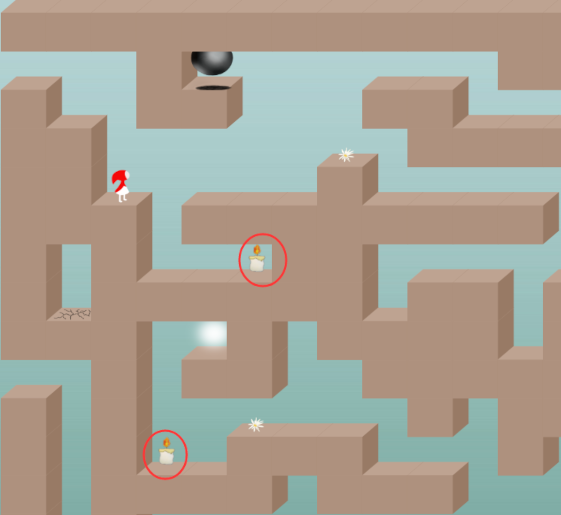
\includegraphics[height=\heightiii]{candle2}};
		\node[anchor=south west,outer sep=0pt,inner sep=0pt] at (c2.north west) {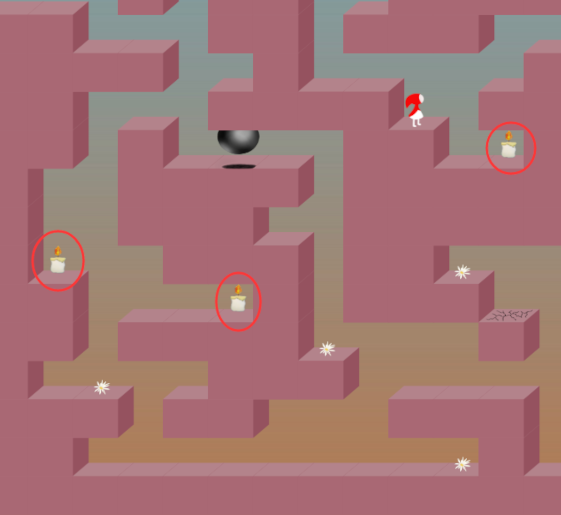
\includegraphics[height=\heightiii]{candle3}};

	\end{tikzpicture}
	\begin{columns}
		\column{.22\textwidth}

		\column{.7275\textwidth}
		Comments:
		\begin{itemize}\bigsep
			\item Three pictures
			\item On the left (west)
			\item Too small for more than three pictures
			\item Ensure all pictures have the exact same size
		\end{itemize}
	\end{columns}

\end{frame}

\begin{frame}[t]{Three pictures}

	\begin{tikzpicture}[overlay, remember picture]

		\node[anchor=south west,outer sep=0pt,inner sep=0pt] (c1) at (current page.south west)  {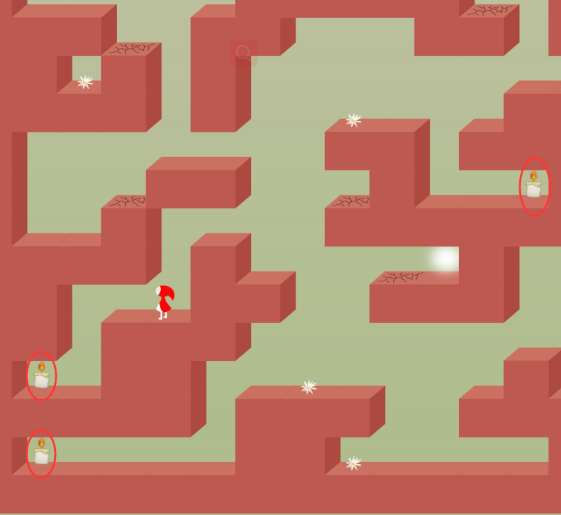
\includegraphics[width=\widthiii]{candle1}};
		\node[anchor=south west,outer sep=0pt,inner sep=0pt] at (c1.south east) (c2) {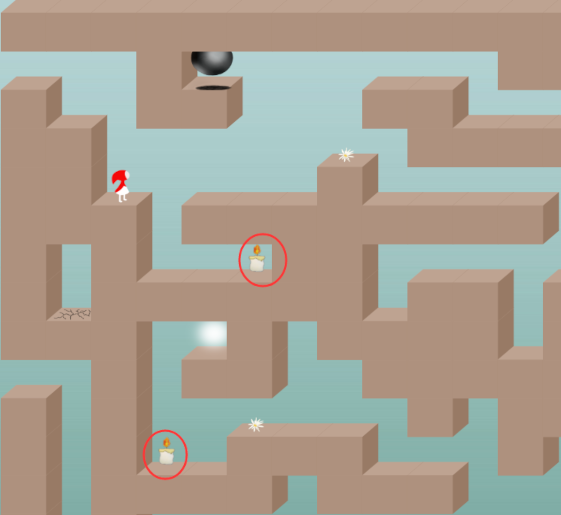
\includegraphics[width=\widthiii]{candle2}};
		\node[anchor=south west,outer sep=0pt,inner sep=0pt] at (c2.south east) {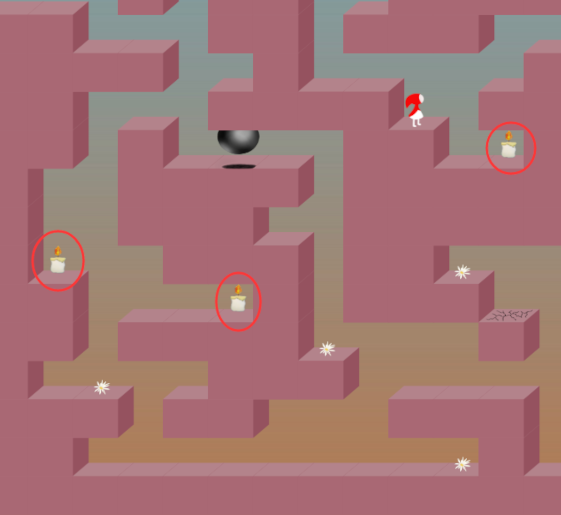
\includegraphics[width=\widthiii]{candle3}};

	\end{tikzpicture}

	Comments:
	\begin{itemize}
		\item Three pictures
		\item On the bottom (south)
		\item Notice the {\tt [t]} when using the frame environment
	\end{itemize}

\end{frame}

\begin{frame}{Faded pictures}

		\begin{columns}
			\column{\halfwidth}
			\fadedpic[width=\textwidth]{candle1}{Short caption}
			\column{\halfwidth}
			\fadedpic[width=\textwidth]{candle3}{Longer caption over more than one line}
		\end{columns}
		\pause
	Slide content:
	\begin{itemize}
		\item Background is shown on the first overlay 
		\item For all other overlays its opacity is lowered
		\item Text can be written atop of the image
	\end{itemize}
\end{frame}

\section{Make a character speak}

\begin{frame}

	\begin{tikzpicture}

		\node at (0,0) {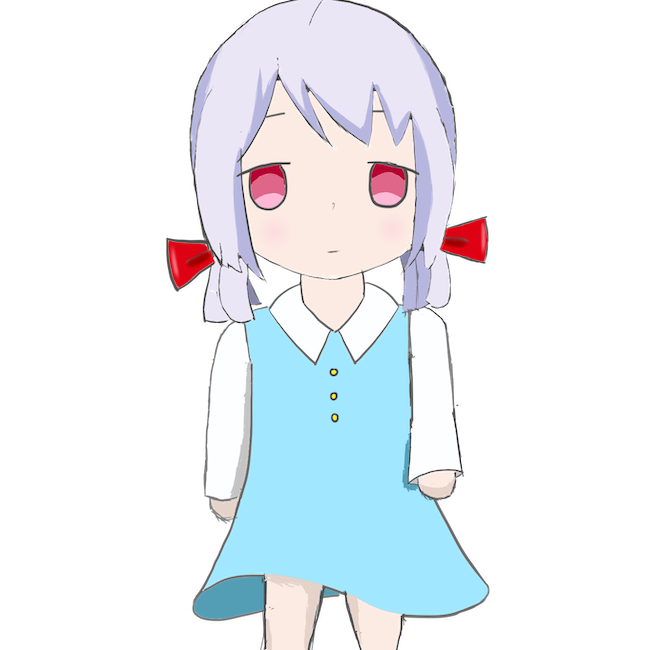
\includegraphics[scale=.2]{sonia.png}};

		\onslide<1>{
			\node[shape=ellipse callout, callout absolute pointer={(.15,.5)}, draw, align=center, text width=3cm, fill=blue!5, draw=black!65, text=blue!75 ] at (3.25,1.6) {My name is Sonia, an ordinary girl in the town, maybe.}; 
		}
		\onslide<2>{
			\node[shape=cloud callout, cloud puffs=15, cloud puff arc=100, callout pointer segments=2,aspect=2.5, callout relative pointer={(200:1.25)}, draw, align=center, text width=3cm, fill=pink!10, draw=black!45, text=black ] at (3.5,3.5) {Why did I say ``maybe?''}; 
		}
		\onslide<3>{
			\node[shape=rectangle callout, callout absolute pointer={(0.15,.5)}, draw, align=center, text width=3cm, fill=red!5, fill opacity=.5, text opacity=1, draw=black!65 ] at (2.2,2) {Oh, no! Where are my legs?}; 
		}
	\end{tikzpicture}

\end{frame}

\begin{frame}{Comments}

	Basic animations:
	\begin{itemize}
		\item Animations that support your words are good
		\item Avoid useless fancy transitions and animations:
			\begin{itemize}
				\item They do not add anything to your message 
				\item They simply distract the audience
			\end{itemize}
		\item Notice that Sonia does not move between two bubbles
		\item The three Sonia are on a same slide but different overlays  
	\end{itemize}

\end{frame}

\section{Embedding documents}

\begin{frame}{Include a video}

	Playing videos:
	\begin{itemize}\bigsep
		\item The video must be in the same directory as the slides 
		\item Manually take a screenshot of the video and display it
		\item Ensure your PDF reader can play videos
		\item In zoom ensure you also share the sound
	\end{itemize}

\end{frame}


\begin{framem}{}

	\tikz[remember picture, overlay]\node at (current page.center) {\href{run:trailer.mp4}{\XeTeXLinkBox{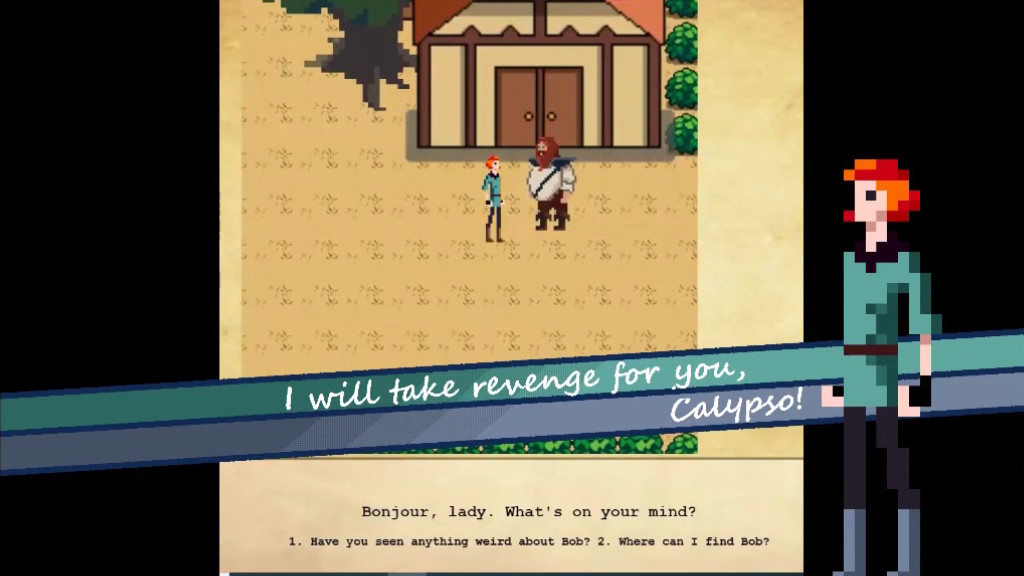
\includegraphics[width=\paperwidth,keepaspectratio]{trailer}}}};

\end{framem}

\begin{frame}{Spy on a poster}

	Basic guidelines:
	\begin{itemize}
		\item Transform the PDF into a JPEG file:
		\begin{itemize}
			\item Width should be about 3000 px
			\item Quality should be 90\% 
			\item Ensure the zoomed content remains sharp
		\end{itemize}
		\item Many shapes are available (refer to tikZ documentation)
		\item Refer to the source code for detailed comments
%		\item Do not forget to add {\tt \textbackslash usetikzlibrary\{spy\}} to the preamble
	\end{itemize}
		
\end{frame}


\setslidecolor{bg=black}
\begin{frame}

	\begin{tikzpicture}[spy using outlines={magnification=1.8, connect spies},white!90!black, remember picture, overlay,anchor=north west]

		% default anchor was changed above to north west (top left corner)
		% reset it to center 
		\node[anchor=center] at (current page.center) {\pgfimage[width=\paperwidth]{poster}};

		% specify the height/width around the box: exactly select the right size, or "far too much" (to not make the audience feel you badly selected your box)
		% the 2 are shown below ("too large" one is much harder to fit...)
		% process: find the coordinates of the top left corner, then adjust h/w
		% anchor of the zoom version might be adjusted to obtain the proper alignment, below east "means" align right 
		\only<2>{\spy[rounded corners=10pt,height=2.6cm, width=5.65cm] on (-.025,-3.425) in node[anchor=east] at (11.1,0);}
		\only<3>{\spy[tape,width=7.44cm, height=3.61cm] on (.735,-1.16) in node[anchor=east] at (11.1,1.5);}
		\only<4>{\spy[cloud,width=6.4cm, height=4.61cm] on (6.665,-.725) in node[anchor=east] at (5.5,1.4);}

	\end{tikzpicture}

\end{frame}

\resetslidecolor

\begin{framek}

	\begin{itemize}\itemsep .5cm
		\item Summary of the main features of the game
		\item This slide is optional, remove it if you wish
	\end{itemize}

\end{framek}

\end{document}
